\section{Experiments}\label{chapter4}

\subsection{Dataset}
We illustrate our two \textsc{nmf} algorithms on two real-world face image datasets: ORL and Extended YaleB (\citet{belhumeur1997eigenfaces}). 
Both ORL and Extended YaleB datasets contain multiple images of distinct subjects with various facial expression, lighting condition, and facial details. 
Images in ORL are cropped and resized to $92 \times 112$ pixels. We further rescale it to $30 \times 37$ pixels. Similarly, we reduce the size of images in Extended YaleB to $42 \times 48$ pixels.
For each dataset, we flatten the image matrix into a vector and append them together to get a matrix $V$ with shape $(d, n)$ where $d$ is the number of pixels in one image and $n$ is the number of images. In each epoch, we use 90\% of data. 

\subsection{Noise}
We implement three kinds of noises including Gaussian noise, Poisson noise and Salt \& Pepper noise.
\subsubsection{Gaussian Noise}\label{sec:gau}
We design the Gaussian noise by normal distribution with $0$ mean and $80$ standard deviation (Algorithm~\ref{gau}). The \texttt{ORL} dataset has a global pixel mean of $40$ and the \texttt{CroppedYale} data set has that of $70$. Hence the designed Gaussian noise contaminates the images significantly. We choose the standard deviation to be $80$ so that our Gaussian noise are less likely to coincident with the designed Poisson noise. To satisfy the nonnegative constant, negative value in contaminated image is set to zero
\begin{lstlisting}[caption= Gaussian Noise Design, label=gau]
def normal(subVhat):
    """Design a Gaussian noise."""
    V_noise = np.random.normal(0, 80, subVhat.shape) #* np.sqrt(subVhat)
    V = subVhat + V_noise
    V[V < 0] = 0
    return V, V_noise
\end{lstlisting}


\subsubsection{Poisson Noise}\label{sec:poi}
The Poisson noise is not additive and has no hyperparameters to be set. Unlike Gaussian noise, contaminated images are drawn directly from Poisson distribution with parameter set to be pixel values. Then, the Poisson noise is calculated from the difference between the contaminated image and the original image, as discussed in Section~\ref{chapter2} and demonstrated in algorithm~\ref{poi}.
\begin{lstlisting}[caption= Poisson Noise Design, label=poi]
def possion(subVhat):
    """Design a Possion noise."""
    V = np.random.poisson(subVhat)
    V_noise = V-subVhat
    return V, V_noise
\end{lstlisting}


\subsubsection{Salt \& Pepper Noise}\label{sec:sal}
% JOYCE please add here
Salt and Pepper noises are added by drawing random integers from discrete uniform distribution of the interval $[$0, 255$)$ \chenc{joyce please comment here about your noise.} ref~\ref{salt}
\begin{lstlisting}[caption= Salt and Pepper Noise Design, label=salt]
"""Design a salt and pepper noise where make some pixel value zeros."""
  V_noise = np.random.randint(low=0, high=255, size=subVhat.shape, dtype=int)
  V = subVhat.copy()
  V[V_noise <= 20] = 0
  V[V_noise >= 230] = 255
  return V, V_noise
\end{lstlisting}

\subsection{Experiments Results}
Figure~\ref{noisesnmf} and~\ref{noisesklnmf} visualise the original image, designed noises, corrupted images and reconstructed images from left to right. From top to bottom, the four rows correspond to no noise, Gaussian noise discussed in Section~\ref{sec:gau}, Poisson noise discussed in Section~\ref{sec:poi} and Salt \& Paper noise discussed in Section~\ref{sec:sal}. {\color{blue} SOMEONE PLEASE DESCRIBE THE IMAGE HERE.}

Kolmogorov-Smirnovs test compare the \textsc{rre}s between the two algorithm gives test statistics $D=1,1,0.6625>0.215$ with no noise, Gaussian noise, and Poisson noise, for the \textsc{orl} dataset. Hence there are strong evidence that the performance of \textsc{nmf} and \textsc{klnmf} are different in these three problems. For salt and Pepper noise, test statistic~$D=0.2125<0.215$, hence we fail to conclude that the two methods have different robustness against Salt and Pepper noise. Further one tail Kolmogorov-Smirnov test concludes that \textsc{klnmf} performs better reconstructing the original image with no noise and is more robust Poisson noise. 
In contrast, \textsc{nmf} is more robust against Gaussian noise, even with only $500$ iterations ($1200$ for \textsc{klnmf}). Hence, \textsc{nmf} is clearly more robust than \textsc{klnmf} against Gaussian noise. 

Theoretical results discussed in Section~\ref{chapter2} suggest \textsc{nmf} is more robust against Gaussian noise whereas \textsc{klnmf} is more robust against Poisson noise. Our experimental results concluded from Kolmogorov-Smirnovs hypothesis tests agree with these theoretical results. Further, as both of the algorithms are not designed for Salt and Pepper noise, they have similar performance against it.

These results can be observe by directly reading the confidence intervals in table~\ref{tab:ci}. Also, the statistical results agree with the visualisation in Figure~\ref{noisesnmf}.

In terms of the cropped Yale dataset, results from hypothesis tests show that \textsc{nmf} performs uniformly better than \textsc{klnmf}, suggesting more iterations are required on \textsc{klnmf} to compare these two algorithms fairly. We fail to do so because the dataset is much larger than \textsc{orl} and our multiplicative update rules, especially for \textsc{klnmf} converge too slow.

\begin{figure}\label{noisesnmf}
	\centering
	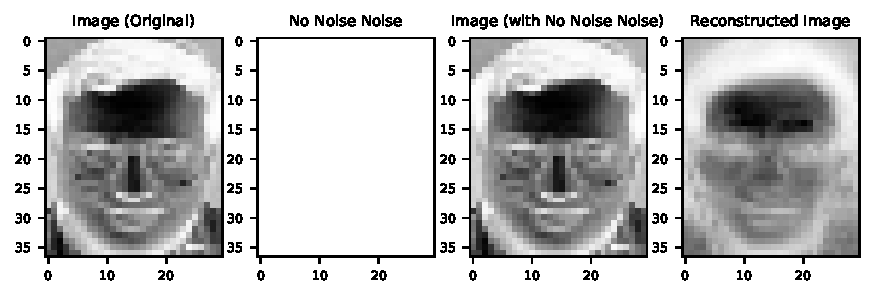
\includegraphics[scale=.9]{Result_Multiplication_Euclidean_No_Noise_Comparison}\\
	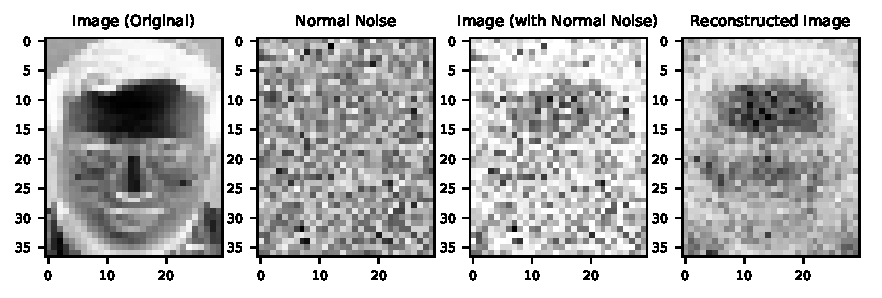
\includegraphics[scale=.9]{Result_Multiplication_Euclidean_Normal_Comparison}\\
	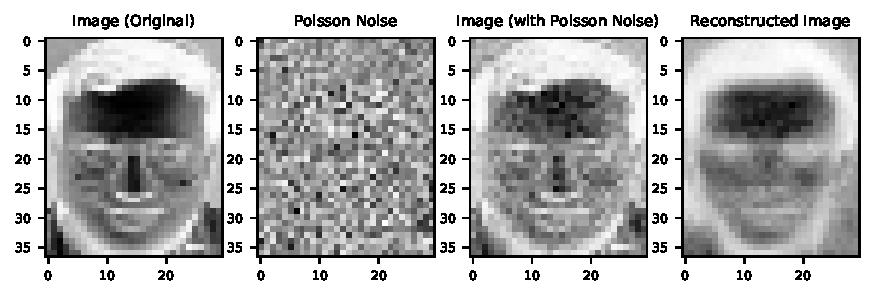
\includegraphics[scale=.9]{Result_Multiplication_Euclidean_Poisson_Comparison}\\
	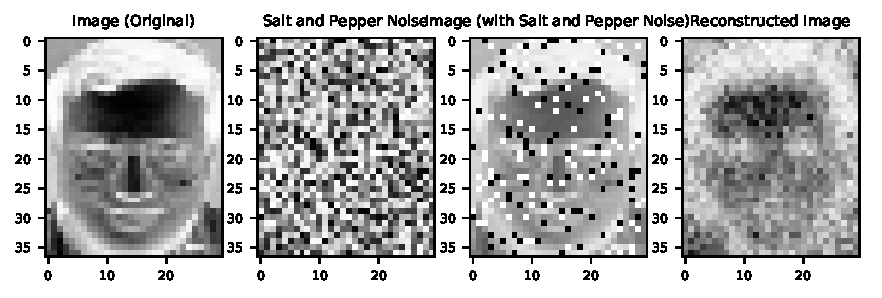
\includegraphics[scale=.9]{Result_Multiplication_Euclidean_Salt_and_Pepper_Comparison}
	\caption{The reconstructed image by \textbf{nmf}. The original images (Column~1) are combined with noises (Column~1) including Gaussian Noise with Variance~$80$ (Row~2), Poisson Noise (Row~3), and Salt \& Pepper Noise (Row~4). The corrupted images are shown in Column~3. The reconstructed image are shown in (Column~4). The reconstruction with no noise is shown in Row~1.}
	\label{fig:noise}
\end{figure}
\begin{figure}\label{noisesklnmf}
	\centering
	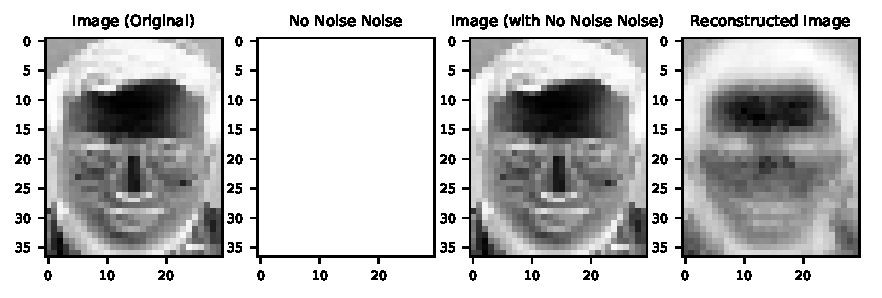
\includegraphics[scale=.9]{Result_Multiplication_KL_Divergence_No_Noise_Comparison}\\
	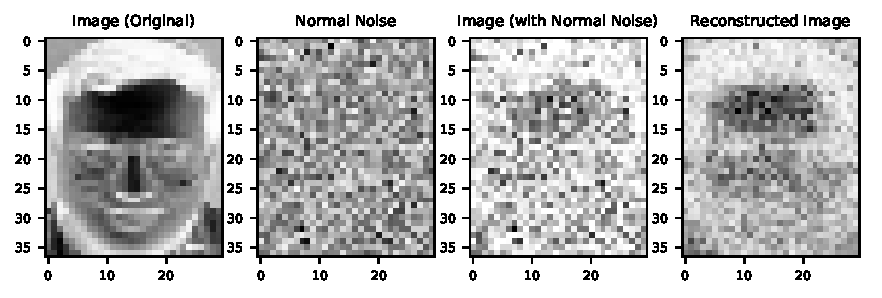
\includegraphics[scale=.9]{Result_Multiplication_KL_Divergence_Normal_Comparison}\\
	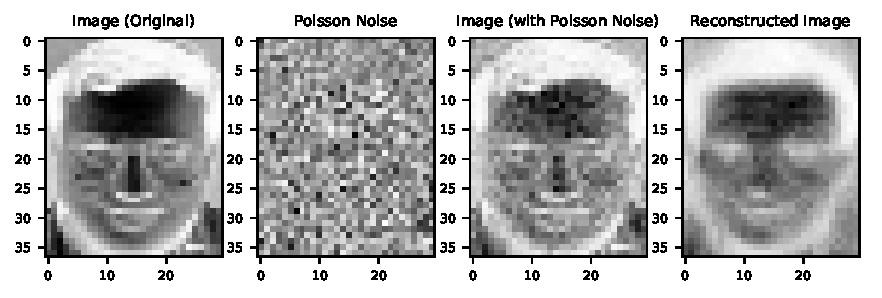
\includegraphics[scale=.9]{Result_Multiplication_KL_Divergence_Poisson_Comparison}\\
	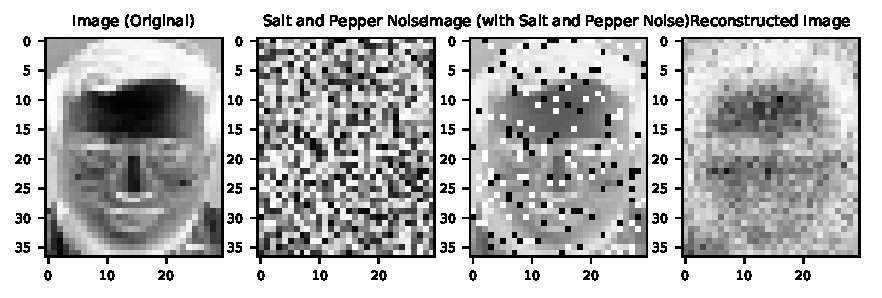
\includegraphics[scale=.9]{Result_Multiplication_KL_Divergence_Salt_and_Pepper_Comparison}
\caption{The reconstructed image by \textbf{klnmf}. The original images (Column~1) are combined with noises (Column~1) including Gaussian Noise with Variance~$80$ (Row~2), Poisson Noise (Row~3), and Salt \& Pepper Noise (Row~4). The corrupted images are shown in Column~3. The reconstructed image are shown in (Column~4). The reconstruction with no noise is shown in Row~1.}
	\label{fig:noise}
\end{figure}

\begin{table}
\caption{Average of evaluations metrics over 80 simulations using the \textsc{orl} dataset. The 95\% confidence intervals are calculated using bootstrap.}
\hspace{-1cm}{\small
\label{tab:ci}\begin{tabular}{l|lll}
 \hline
\textsc{orl} dataset & \textsc{rre} & \textsc{acc} & \textsc{nmi}\tabularnewline 
 \hline
\textsc{nmf} no noise & 0.1583 (0.1581, 0.1584) & 0.7364 (0.731, 0.742) & 0.8536 (0.8506, 0.8567)\tabularnewline
 
\textsc{nmf} Gaussian noise & 0.2925 (0.2922, 0.2927) & 0.447 (0.4423, 0.4521) & 0.6212 (0.6176, 0.6247)\tabularnewline
 
\textsc{nmf} Poisson noise & 0.1611 (0.161, 0.1613) & 0.7313 (0.7262, 0.7367) & 0.8493 (0.8456, 0.8527)\tabularnewline
 
\textsc{nmf} Salt and Pepper noise & 0.2636 (0.2634, 0.2638) & 0.5094 (0.504, 0.5151) & 0.6721 (0.6679, 0.6764)\tabularnewline
 
\textsc{klnmf} no noise & 0.1729 (0.1728, 0.173) & 0.7406 (0.7352, 0.7458) & 0.8599 (0.8568, 0.8632)\tabularnewline
 
\textsc{klnmf} Gaussian noise & 0.2977 (0.2976, 0.2979) & 0.4538 (0.4483, 0.4595) & 0.6209 (0.6165, 0.6255)\tabularnewline
 
\textsc{klnmf} Poisson noise & 0.1602 (0.1601, 0.1603) & 0.7417 (0.7365, 0.7472) & 0.8573 (0.8542, 0.8602)\tabularnewline
 
\textsc{klnmf} Salt and Pepper noise & 0.264 (0.2638, 0.2643) & 0.5089 (0.5038, 0.5139) & 0.6734 (0.6694, 0.6779)\tabularnewline
 \hline
\end{tabular}}
\end{table}

\subsubsection{{CroppedYale} Evaluations metrics FAKE FOR NOW}
\begin{table}
\caption{Average of evaluations metrics over 40 simulations using CroppedYale data set. The 95\% confidence intervals are calculated using bootstrap.}
\hspace{-1cm}{\small
\begin{tabular}{l|lll}
 \hline
\textsc{orl} dataset & \textsc{rre} & \textsc{acc} & \textsc{nmi}\tabularnewline 
 \hline
\textsc{nmf} no noise & 0.1583 (0.1581, 0.1584) & 0.7364 (0.731, 0.742) & 0.8536 (0.8506, 0.8567)\tabularnewline
 
\textsc{nmf} Gaussian noise & 0.2925 (0.2922, 0.2927) & 0.447 (0.4423, 0.4521) & 0.6212 (0.6176, 0.6247)\tabularnewline
 
\textsc{nmf} Poisson noise & 0.1611 (0.161, 0.1613) & 0.7313 (0.7262, 0.7367) & 0.8493 (0.8456, 0.8527)\tabularnewline
 
\textsc{nmf} Salt and Pepper noise & 0.2636 (0.2634, 0.2638) & 0.5094 (0.504, 0.5151) & 0.6721 (0.6679, 0.6764)\tabularnewline
 
\textsc{klnmf} no noise & 0.1729 (0.1728, 0.173) & 0.7406 (0.7352, 0.7458) & 0.8599 (0.8568, 0.8632)\tabularnewline
 
\textsc{klnmf} Gaussian noise & 0.2977 (0.2976, 0.2979) & 0.4538 (0.4483, 0.4595) & 0.6209 (0.6165, 0.6255)\tabularnewline
 
\textsc{klnmf} Poisson noise & 0.1602 (0.1601, 0.1603) & 0.7417 (0.7365, 0.7472) & 0.8573 (0.8542, 0.8602)\tabularnewline
 
\textsc{klnmf} Salt and Pepper noise & 0.264 (0.2638, 0.2643) & 0.5089 (0.5038, 0.5139) & 0.6734 (0.6694, 0.6779)\tabularnewline
 \hline
\end{tabular}}
\end{table}